\subsection{Objekt vs. Klasse}

Der Objektbegriff in der Softwareentwicklung umfasst Dinge, die man sehen und/oder anfassen kann, wie zum Beispiel eine Katze, einen Tisch, eine Person oder einen Stern, aber auch immaterielle Dinge, wie zum Beispiel ein Konto, eine Reise oder eine Vorlesung. In der objektorientierten Softwareentwicklung werden die (zukünftigen) Objekte\marginpar{Objekt} eines Softwaresystems von Objekten der Realwelt abgeleitet. Abhängig vom Einsatzzweck der Software werden bei der Bestimmung der systeminternen Objekte bestimmte Eigenschaften der Realwelt-Objekte berücksichtigt und andere ignoriert, so dass nur die für die zukünftige Software relevanten Eigenschaften der Realwelt-Objekte betrachtet werden. System-Objekte sind damit Abstraktionen von Realwelt-Objekten.

Ein System-Objekt hat eine eindeutige Identität, die es von anderen Objekten des Systems unterscheidbar macht. Es verfügt über Eigenschaften, kann wechselnde Zustände annehmen und bietet anderen Objekten eine Menge an Operationen an. In Reaktion auf den Aufruf seiner Operationen zeigt das Objekt ein bestimmtes Verhalten. Dabei kann es sich zum Beispiel um die Änderung seines Zustandes oder den Aufruf weiterer (eigener oder fremder) Operationen handeln. In der UML werden Objekte als rechteckige Kästen dargestellt, die (mindestens, s.u.) den Objektnamen\footnote{Der Objektname ist nicht gleichzusetzen mit der Identität des Objektes. Der Name ist lediglich ein Bezeichner, der das Objekt innerhalb eines Diagramms identifiziert, aber nicht im gesamten System.} enthalten (Abb.~\ref{fig:Abb-3-2}).
\begin{wrapfigure}{o}[70pt]{0.6\textwidth}
	%\vspace{-10pt}
	\centering 
	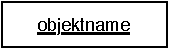
\includegraphics{../grafiken/Kapitel-3/Abb-3-2.pdf}
	\caption{Ein Objekt in UML-Darstellung}
	\label{fig:Abb-3-2}
	\vspace{-6pt}
\end{wrapfigure}
Nach UML-Konvention wird der Objektname unterstrichen dargestellt. Üblich – obwohl die UML diesbezüglich keine Vorgaben macht – ist außerdem, dass Objektnamen mit einem Kleinbuchstaben beginnen und zentriert dargestellt werden. Innerhalb eines Diagramms müssen die Objektnamen eindeutig gewählt werden. Sollten innerhalb eines Diagramms trotzdem zwei Kästchen denselben Namen enthalten – die UML verbietet dies nicht – so ist per Definition mit beiden Kästchen dasselbe Objekt gemeint. Die Darstellung als zwei Kästchen wird vor allem in handschriftlich erstellten Diagrammen aus Lesbarkeitsgründen verwendet.

\begin{wrapfigure}{o}[70pt]{0.6\textwidth}
	%\vspace{-10pt}
	\centering 
	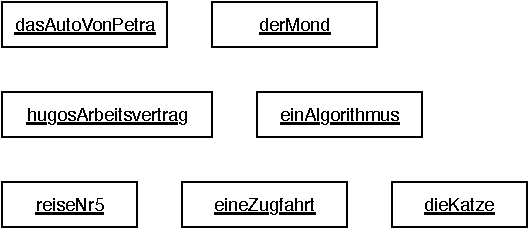
\includegraphics{../grafiken/Kapitel-3/Abb-3-3.pdf}
	\caption{Einige Objekte}
	\label{fig:Abb-3-3}
	\vspace{-6pt}
\end{wrapfigure}
Abbildung~\ref{fig:Abb-3-3} zeigt einige Objekte in UML-Darstellung.
Bei manchen wird aus dem Namen (relativ) deutlich, welches konkrete Realwelt-Objekt sie abbilden sollen. So ist \texttt{dasAutoVonPetra}, sofern man Petra kennt und sie nicht mehr als ein Auto besitzt, einem konkreten Realwelt-Auto zuordenbar. Für \texttt{reiseNr5} bedarf es dagegen schon der zusätzlichen Kenntnis des Kontextes (z.B. die Auflistung von Reisen in einem Katalog), um eine Realwelt-Reise mit diesem Namen zu verbinden. Für Objekte wie \texttt{einAlgorithmus} oder \texttt{eineZugfahrt} und auch \texttt{dieKatze} schließlich lassen sich die gemeinten Realwelt-Entsprechungen nicht bestimmen. Zumindest könnte man anhand der Namen der Objekte aber vielleicht auf die Art des Realwelt-Objektes schließen. So sollte es sich bei \texttt{dieKatze} doch wohl um eine Katze und nicht um einen Hund handeln.


Doch vielleicht trägt mein Meerschweinchen – aus welchem Grund auch immer – den Namen \texttt{dieKatze} und meine Katze heißt stattdessen \texttt{pünktchen}. \begin{wrapfigure}{o}[70pt]{0.7\textwidth}
	%\vspace{-10pt}
	\centering 
	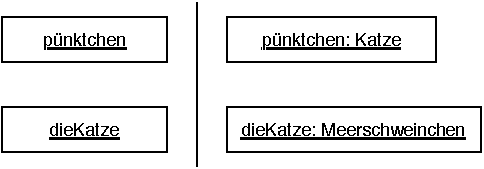
\includegraphics{../grafiken/Kapitel-3/Abb-3-4.pdf}
	\caption{Links: Ein Objekt namens \texttt{pünktchen} und ein Objekt namens \texttt{dieKatze}. Rechts: Ein Katzen-Objekt namens \texttt{pünktchen} und ein Meerschweinchen-Objekt namens \texttt{dieKatze}}
	\label{fig:Abb-3-4}
	\vspace{-6pt}
\end{wrapfigure}
Um solche Sachverhalte unmissverständlich zu modellieren, wird neben dem Objektnamen noch die Information benötigt, um welche Art von Objekt es sich handelt. In der UML-Darstellung eines Objektes wird dafür der Objektname um die Angabe des Namens der so genannten Klasse ergänzt (Abb.~\ref{fig:Abb-3-4} rechts). Die Objektdarstellung ohne zusätzlichen Klassennamen (wie in Abb.~\ref{fig:Abb-3-2} und Abb.~\ref{fig:Abb-3-3}) ist nach UML-Regeln zulässig, sollte aus semantischen Gründen aber nur dann verwendet werden, wenn aus dem Kontext eindeutig auf den Typ (die zugehörige Klasse) des Objektes geschlossen werden kann.

Das Konzept der Klasse\marginpar{Klasse} ist ein wichtiger Bestandteil der objektorientierten Softwareentwicklung.\footnote{Auch wenn es einige wenige objektorientierte Programmiersprachen gibt (z.B. Javascript, Go), die keine Klassen, sondern nur Objekte kennen.} Aus einer konzeptuellen Sicht gruppiert eine Klasse eine Menge von System-Objekten anhand identifizierter Gemeinsamkeiten. So können zum Beispiel alle System-Objekte, die Realwelt-Katzen modellieren, der Klasse Katze zugeordnet werden, während System-Objekte, die Realwelt-Meerschweinchen abbilden, zur Klasse Meerschweinchen gehören. Eine Klasse definiert, welche Aspekte der Objekte für ihre Zugehörigkeit zur Klasse relevant sind. So könnte es zum Beispiel notwendig sein, dass ein Objekt schnurren kann, um vom Typ Katze zu sein, wogegen es irrelevant ist, welche Farbe das Fell hat oder vielleicht auch, ob das Objekt überhaupt ein Fell hat (Nacktkatzen). Klassen sind somit Abstraktionen von System-Objekten. Sie abstrahieren von der konkreten Ausprägung der Eigenschaften ihrer Objekte (z.B. Farbe des Fells) und den Zuständen, in denen sich ihre Objekte befinden können. Aus Implementierungssicht sind Klassen Schablonen für die Erstellung von System-Objekten. Eine Klasse definiert, welche Eigenschaften, welches Verhalten und welche Beziehungen zu anderen Objekten die ihr zugehörigen Objekte aufweisen sollen. Eine Klasse definiert außerdem einen Mechanismus – in der objektorientierten Programmierung als Konstruktor bezeichnet – über den neue Objekte vom Typ der Klasse erzeugt werden können. Jedes zur Laufzeit der Software benötigte Objekt einer Klasse wird so anhand der Vorgaben der Klasse konstruiert.

Diese Erzeugung neuer Objekte einer Klasse nennt man Instanziierung und statt vom Objekt der Klasse spricht man in diesem Zusammenhang von der Instanz der Klasse. Einen inhaltlichen Unterschied zwischen den Begriffen Instanz und Objekt gibt es nicht. Der Begriff Instanz wird verwendet, wenn die Zugehörigkeit eines Objektes zu seiner Klasse wichtig ist („Eine Instanz der Klasse Katze“), weil damit zum Beispiel ausgedrückt werden soll, dass dieses konkrete Objekt alle Eigenschaften besitzt, die die entsprechende Klasse definiert hat. Der Begriff Objekt wird in allgemeineren Zusammenhängen verwendet. Eine scharfe Trennlinie gibt es aber nicht. Letztendlich können die Begriffe synonym verwendet werden – und werden sie in der Literatur auch häufig. Die Menge aller zu einem Zeitpunkt existierenden Instanzen einer Klasse bezeichnet man mit dem Begriff der Extension. 

Die UML-Darstellung einer Klasse ist sehr ähnlich zu der Darstellung eines Objektes. Es handelt sich ebenfalls um ein Rechteck, in dem (mindestens, s.u.) der Klassenname eingetragen ist.
\begin{wrapfigure}{o}[70pt]{0.7\textwidth}
	%\vspace{-10pt}
	\centering 
	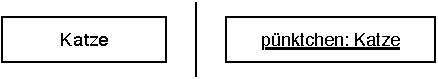
\includegraphics{../grafiken/Kapitel-3/Abb-3-5.pdf}
	\caption{Eine Klasse mit Namen \texttt{Katze} (links) und eine Instanz dieser Klasse mit Namen \texttt{pünktchen} (rechts)}
	\label{fig:Abb-3-5}
	\vspace{-6pt}
\end{wrapfigure}
Abbildung~\ref{fig:Abb-3-5} zeigt eine Klasse \texttt{Katze} und eine Instanz namens \texttt{pünktchen} der Klasse Katze. Im Unterschied zu Objekten wird der Name der Klasse nicht unterstrichen. Zudem ist es üblich, den Klassennamen mit einem Großbuchstaben zu beginnen und ihn zentriert und fett gedruckt zu setzen. Der Klassenname ist üblicherweise ein Substantiv im Singular. Abbildung~\ref{fig:Abb-3-6} zeigt weitere Instanzen der Klasse Katze.

Wichtig ist, dass ausschließlich die Angabe \texttt{:Katze} bestimmt, dass es sich um ein Objekt vom Typ Katze handelt. Der Name des Objektes selber sagt nichts über den Typ des Objektes aus. 
\begin{wrapfigure}{o}[70pt]{0.7\textwidth}
	%\vspace{-10pt}
	\centering 
	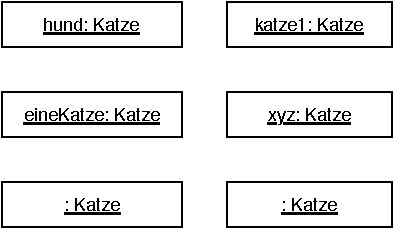
\includegraphics{../grafiken/Kapitel-3/Abb-3-6.pdf}
	\caption{sechs verschiedene Instanzen der Klasse Katze}
	\label{fig:Abb-3-6}
	\vspace{-6pt}
\end{wrapfigure}
So handelt es sich auch bei dem Objekt mit dem Namen \texttt{hund} in Abbildung~\ref{fig:Abb-3-6} um eine Katze. Die beiden unteren Objekte in der Abbildung (\texttt{:Katze}) sind so genannte anonyme Objekte. Diese Form der Darstellung wird verwendet, wenn man nicht eine konkrete, mit einem Namen versehene, Katzen-Instanz modellieren möchte, sondern „irgendein“ Objekt vom Typ Katze. Beachten Sie, dass auch ein anonymes Objekt nur genau \underline{ein} Objekt ist, es steht nicht stellvertretend für alle möglichen Katzen-Instanzen. Im Unterschied zu benannten Instanzen darf es innerhalb desselben Objektdiagramms auch mehrere anonyme Instanzen derselben Klasse geben. Bei diesen handelt es sich dann per Definition um unterschiedliche Objekte. Die beiden anonymen Katzen-Instanzen in Abbildung~\ref{fig:Abb-3-6} modellieren daher zwei unterschiedliche Realwelt-Katzen, bei denen es aber für den Modellierungszweck irrelevant ist, um welche konkreten Realwelt-Katzen es sich handelt. Das Objekt mit Namen \texttt{eineKatze} ist dagegen kein anonymes Objekt sondern modelliert genau diejenige Realwelt-Katze, die den Namen \texttt{eineKatze} trägt.